% Generated by `make loso_plots` from complete baseline masked LOSO runs.
\begin{figure*}[t]
\centering
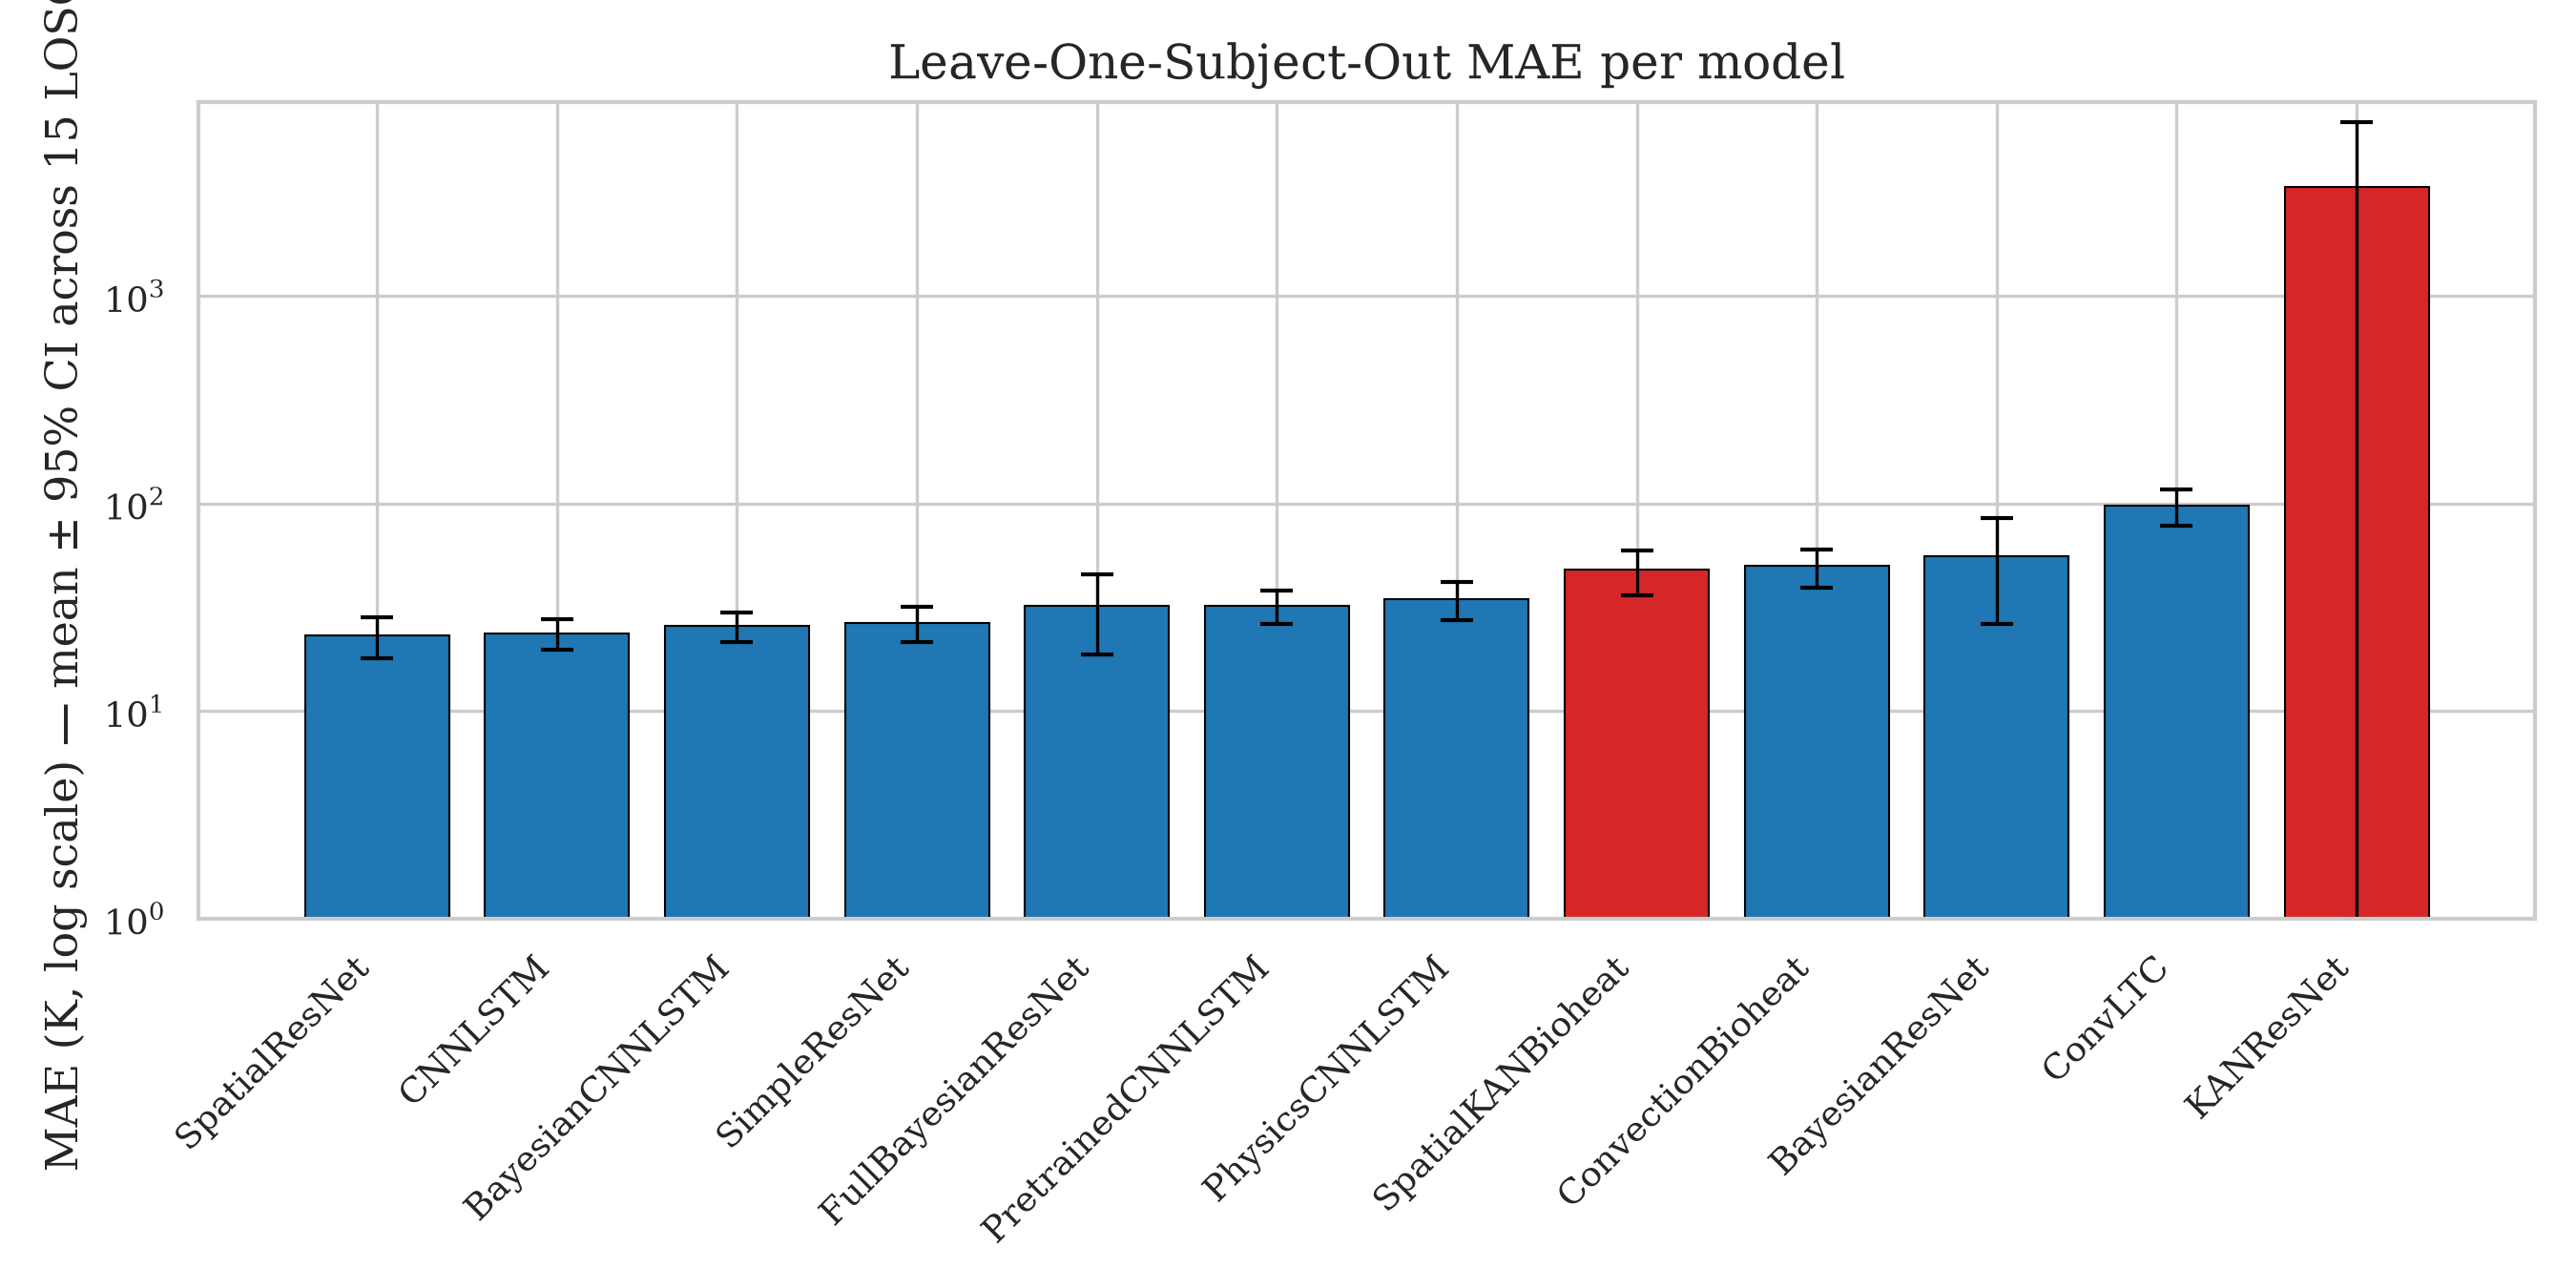
\includegraphics[width=0.78\textwidth]{figures/loso_mae_bars.png}
\caption{Baseline masked LOSO MAE across 15 held-out sequences, ordered by
mean. Error bars show the 95\% confidence interval; the vertical axis is
logarithmic so that the KANResNet divergence does not compress the other
models. The lower confidence bound for KANResNet is clipped at 1\,K for
display.}
\label{fig:loso_mae_bars}
\end{figure*}

\begin{figure*}[t]
\centering
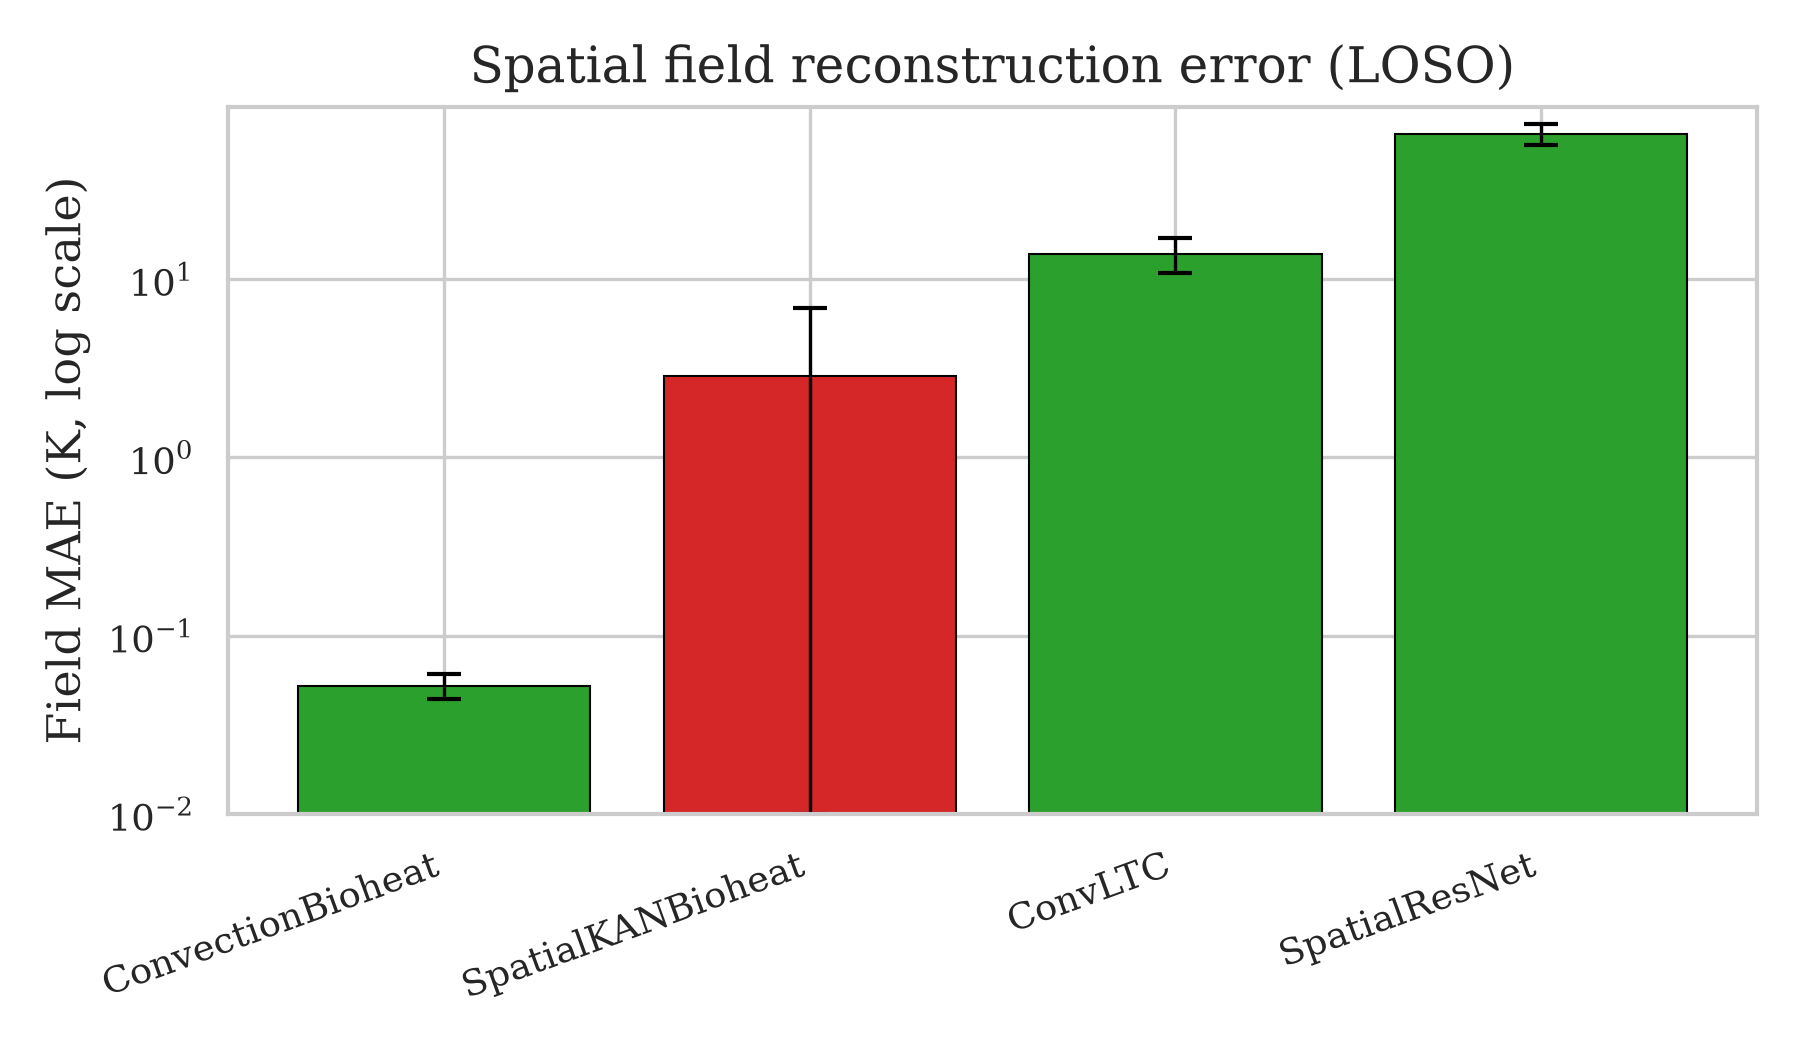
\includegraphics[width=0.82\textwidth]{figures/loso_field_mae_bars.png}
\caption{Spatial field reconstruction MAE on the same LOSO folds (log scale;
lower confidence bounds clipped at 0.01\,K). The
near-zero ConvectionBioheat score (0.05\,K) and low SpatialKANBioheat score
(2.85\,K) are suspicious and should not be interpreted as validated
field-reconstruction accuracy pending investigation of the evaluation
targets.}
\label{fig:loso_field_mae}
\end{figure*}

\begin{figure*}[t]
\centering
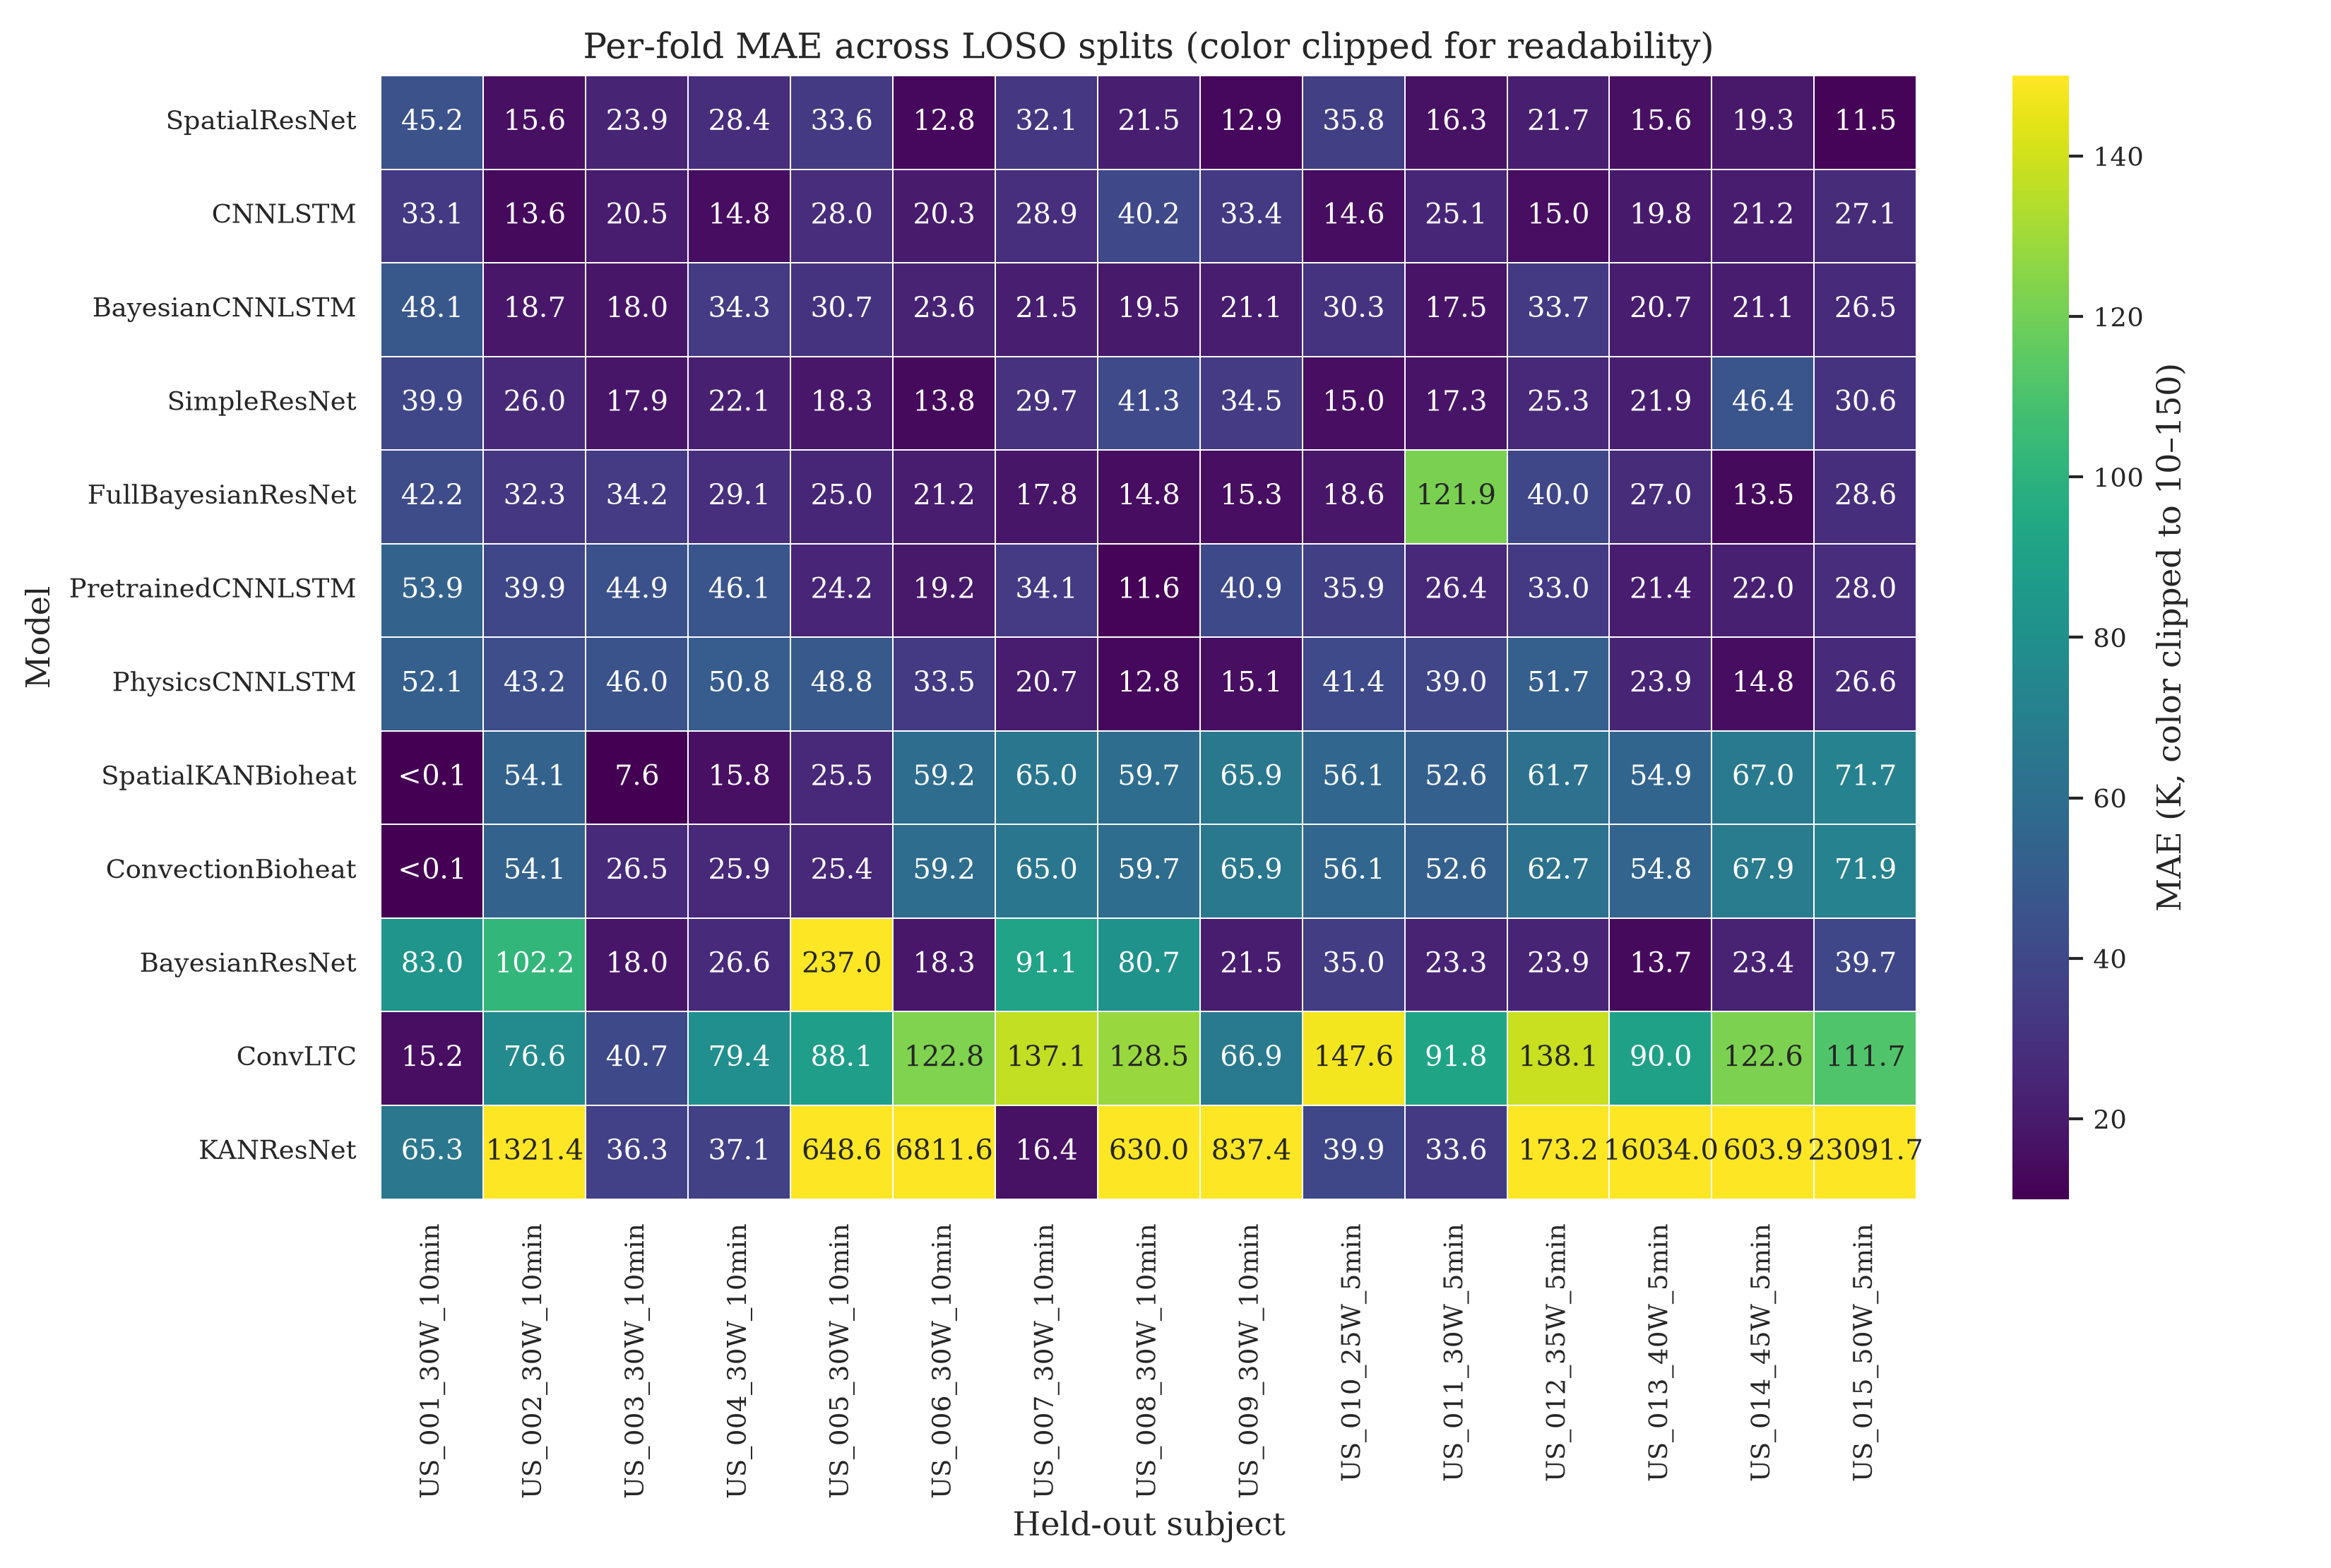
\includegraphics[width=0.92\textwidth]{figures/loso_per_fold_heatmap.png}
\caption{Per-fold baseline masked LOSO MAE (K). Cell labels show the measured
errors; colors are clipped to 10--150\,K so that typical models remain
distinguishable despite the extreme KANResNet outliers.}
\label{fig:loso_per_fold_heatmap}
\end{figure*}

\begin{figure*}[t]
\centering
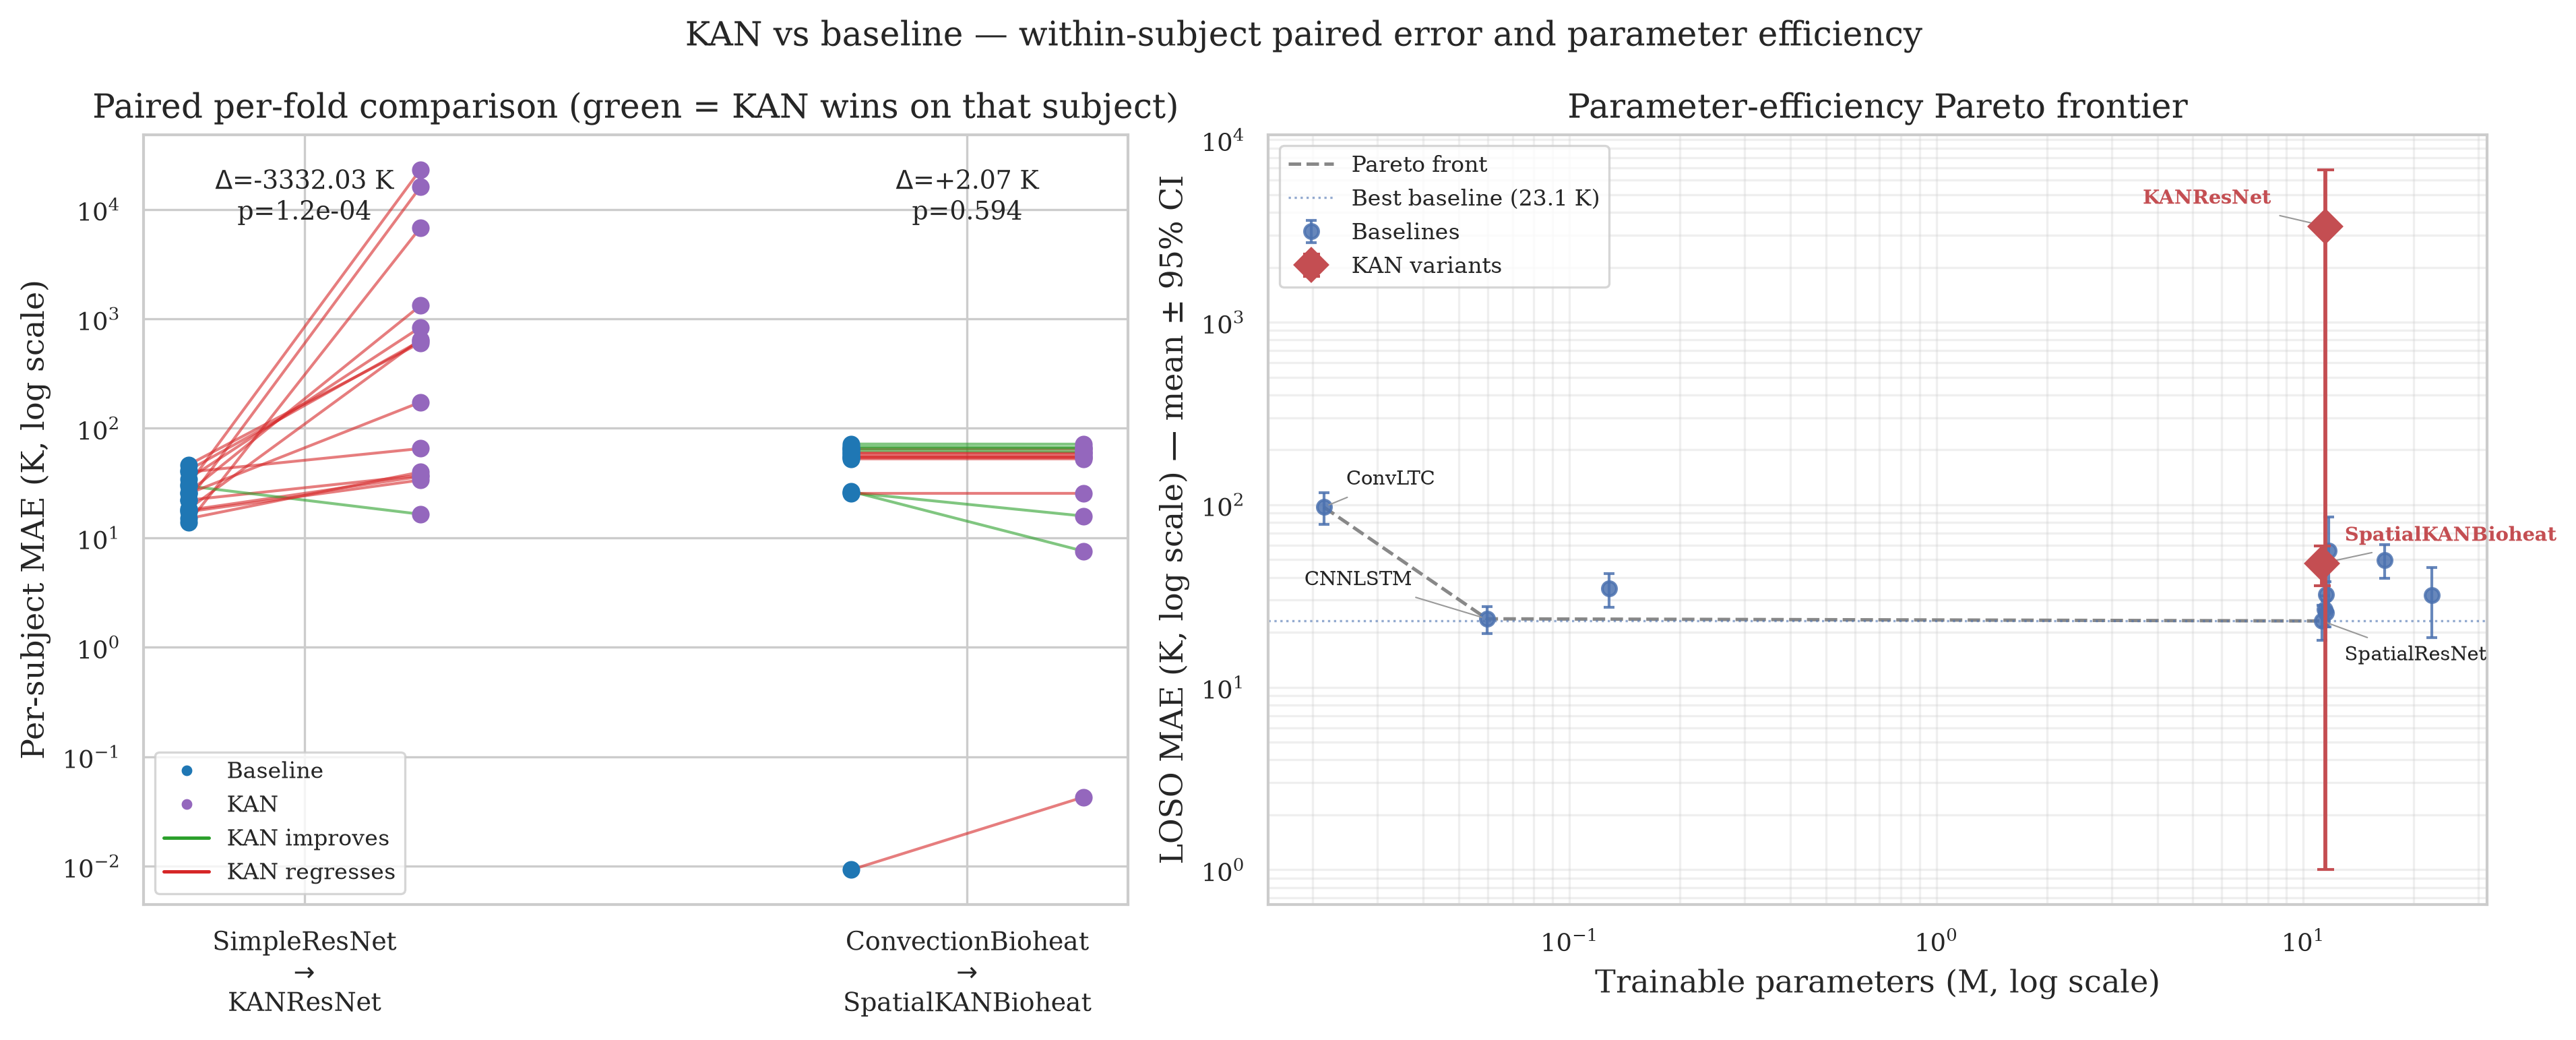
\includegraphics[width=0.96\textwidth]{figures/kan_comparison.png}
\caption{KAN comparison with the baseline architectures. Left: paired
per-fold MAE, with green lines marking folds on which the KAN variant
improves and red lines marking regressions; the vertical axis is logarithmic
to retain the scale of KANResNet divergence. Right: LOSO MAE versus
trainable parameter count, with the Pareto frontier.}
\label{fig:loso_kan_comparison}
\end{figure*}
